% Diese Datei ist Teil des Buchs "Schreibe Dein Programm!"
% Das Buch ist lizensiert unter der Creative-Commons-Lizenz
% "Namensnennung - Weitergabe unter gleichen Bedingungen 4.0 International (CC BY-SA 4.0)"
% https://creativecommons.org/licenses/by-sa/4.0/deed.de

\chapter{Programmieren mit Selbstbezügen und Kombinatoren}
\label{cha:selbstbezug}

Bisher haben wir nur Daten vorgestellt, die
feste Größe haben und damit im Wortsinn beschränkt sind.  Viele
Informationen haben aber variable Größe: Die Bücher im Regal werden
immer mehr, Bauwerke bestehen aus variabel vielen Bauteilen.  Um
solche Informationen als Daten zu repräsentieren, stellen wir in
diesem Kapitel einen weiteren Aspekt der Datenanalyse vor, den
\textit{Selbstbezug}\index{Selbstbezug}.  Hier sind einfache
Beispiele:
%
\begin{itemize}
\item Ein Fluss besteht aus Hauptfluss und Nebenfluss~-- beides wieder
  Flüsse.
\item Ein Dateiverzeichnis auf dem Computer kann 
  Unterverzeichnisse enthalten.
\item Ein großer Bücherstapel besteht aus einem etwas kleineren
  Bücherstapel und einem weiteren Buch.
\end{itemize}
%
Bei all diesen Beispielen werden aus kleineren Dingen größere gemacht:
Aus zwei Flüssen, die zusammenfließen, wird ein großer Fluss.  Aus
mehreren Dateien und Verzeichnissen wird ein großes Verzeichnis.  Aus
einem kleinen Bücherstapel wird ein großer.  In der Programmierung
nennen wir das Bauen von großen Dingen aus kleinen Dingern derselben
Sorte \textit{kombinieren}. Die Funktionen, die das erledigen, heißen
\textit{Kombinatoren}\index{Kombinator}: Um die geht es in diesem Kapitel.

\section{Flüsse abbilden}

\begin{figure}[tbh]
  \centering
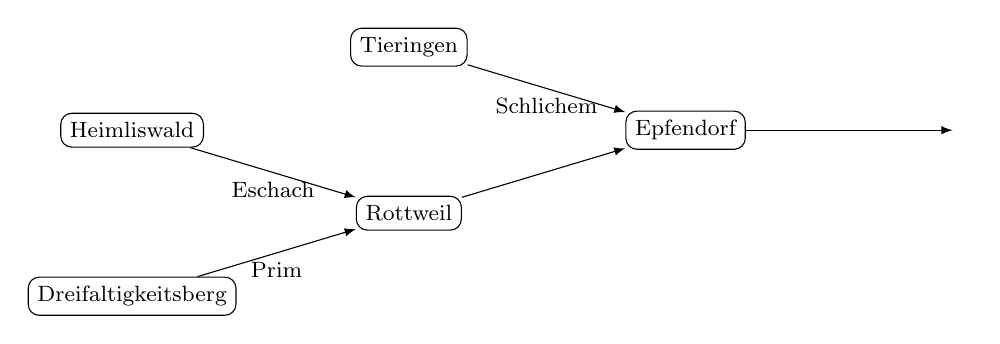
\begin{tikzpicture}
  [
    confluence/.style = {shape=rectangle, rounded corners,
                         draw, align=center},
    absent/.style = {},
    grow                    = left,
    sibling distance        = 6em,
    level distance          = 10em,
    % makes arrows the opposite direction from -latex
    edge from parent/.style = {draw,latex-},
    every node/.style       = {font=\footnotesize}
    ]
    \node [absent] {}
    child {
      node [confluence] {Epfendorf}
        child {
          node [confluence] {Tieringen}
          edge from parent node [below] {Schlichem} }
        child { node  [confluence] {Rottweil}
          child { node [confluence] {Heimliswald}
            edge from parent node [below] {Eschach} }
          child { node [confluence] {Dreifaltigkeitsberg}
            edge from parent node [below] {Prim} } } };
\end{tikzpicture}
  \caption{Der Neckar nahe der Quellen}
  \label{fig:neckar}
\end{figure}

\noindent Abbildung~\ref{fig:neckar} ist ein Diagramm, das die
Struktur des Neckar nahe der Quellen beschreibt: Er fließt zunächst
aus den Bächen Eschach und Prim zusammen, und danach fließen immer
weitere Bäche und Flüsse hinzu~-- in der Abbildung noch die
Schlichem.

Die Struktur eines Flusses werden wir durch Daten abbilden, um danach
eine Funktion zu schreiben, die feststellt, ob ein Fluss durch einen
bestimmten Ort fließt.  Unser erster Versuch einer Datendefinition
sieht so aus:
%
\begin{lstlisting}
; Ein Fluss kommt entweder aus:
; - einer Quelle
; - einem Hauptfluss und einem Nebenfluss
\end{lstlisting}
%
Man kann zwar schon sehen, dass es sich um eine Fallunterscheidung
handelt, aber wir können die Formulierung schärfen, um klar zu machen,
dass es sich um gemischte Daten handelt:
%
\begin{lstlisting}
; Ein Fluss ist eins der folgenden:
; - ein Bach aus einer Quelle
; - ein Zusammentreffen von einem Hauptfluss und einem Nebenfluss
\end{lstlisting}
%
Daraus können wir direkt eine Signaturdefinition machen:
%
\begin{lstlisting}
(define river
  (signature (mixed creek confluence)))
\end{lstlisting}
%
Die Datendefinitionen für "<Bach"> und "<Zusammentreffen"> fehlen
allerdings noch.  In Abbildung~\ref{fig:neckar} steht an den Bächen
jeweils noch der Name.  Eine passende Datendefinition sieht so aus:
%
\begin{lstlisting}
; Ein Bach hat folgende Eigenschaften:
; - Ursprungsort
\end{lstlisting}
%
Das klingt ein bisschen komisch, weil der Bach ja nur \emph{eine}
Eigenschaft hat, aber die Datendefinition trotzdem zusammengesetzte
Daten beschreibt.  Trotzdem ist das legitim und korrekt~-- niemand
wird sagen wollen, dass der Ursprungsort der Bach \emph{ist}.
Außerdem kannst Du Dir vorstellen, dass ein Bach später noch mehr
Eigenschaften bekommt, die wir in den Daten festhalten
wollen. (Wasserqualität oder Fließgeschwindigkeit zum Beispiel.)
Entsprechend ist es auch sinnvoll, dafür eine Record-Definition zu
schreiben:
%
\begin{lstlisting}
(define-record-functions creek
  make-creek
  creek?
  (creek-origin string))
\end{lstlisting}
%
Wenn später noch weitere Eigenschaften hinzukommen, können wir die
Record-Definition erweitern, ohne anderen Code zu beeinträchtigen.

Kommen wir zu den Zusammentreffen.  Auch hier ist ein Ort relevant~--
dort, wo sie zusammentreffen.  Außerdem ist wichtig, \emph{welche}
Flüsse oder Bäche da zusammentreffen.  Die Datendefinition könnte so
aussehen:
%
\begin{lstlisting}
; Ein Zusammentreffen besteht aus:
; - Ort
; - Hauptfluss
; - Nebenfluss
\end{lstlisting}
%
Die Formulierung zeigt eindeutig, dass es sich um zusammengesetzte
Daten handelt.  Aber diese Datendefinition weist eine Auffälligkeit
auf, die erst sichtbar wird, wenn wir sie im Zusammenhang der
Gesamt-Datendefinition für Flüsse betrachten:
%
\tikzstyle{every picture}+=[remember picture]
\tikzstyle{fluss} = [shape=rectangle,inner sep=0pt,text depth=0pt]
%
\begin{lstlisting}
; Ein |\tikz\node[fluss](fluss){\textbf{Fluss}};| ist eins der folgenden:
; - |\ldots|
; - ein Zusammentreffen |\ldots|
|\ldots|
; Ein Zusammentreffen besteht aus:
; - Ort
; - Haupt|\tikz\node[fluss](fluss1){\textbf{fluss}};|
; - Neben|\tikz\node[fluss](fluss2){\textbf{fluss}};|
\end{lstlisting}
%
\begin{tikzpicture}[overlay]
  \path[->,blue,thick](fluss1) edge [out=0, in=0] (fluss);
  \path[->,blue,thick](fluss2) edge [out=0, in=0] (fluss);
\end{tikzpicture}
%
Die Datendefinition für "<Fluss"> benutzt selbst den Begriff
"<Fluss">.   Noch offensichtlicher wird das, wenn wir die dazu
passende Record-Definition erstellen:
%
\begin{lstlisting}
(define-record-functions confluence
  make-confluence
  confluence?
  (confluence-location  string)
  (confluence-main-stem river)
  (confluence-tributary river))
\end{lstlisting}
%
In der Definition von \texttt{confluence} wird \texttt{river} benutzt
und umgekehrt.  Das ist nichts schlimmes~-- im Gegenteil, diese beiden
\textit{Selbstbezüge}\index{Selbstbezug} erlauben uns, ganz
unterschiedliche Flüsse zu beschreiben, insbesondere solche
unterschiedlicher Größe.  Den Abschnitt des Neckar in~\ref{fig:neckar}
können wir so abbilden:
%
\begin{lstlisting}
(define eschach (make-creek "Heimliswald")) ; Quelle des Neckar
(define prim (make-creek "Dreifaltigkeitsberg")) ; Quelle des Neckar
; erster Zusammenfluss des Neckar:
(define neckar-1 (make-confluence "Rottweil" eschach prim))
; Zufluss des Neckar:
(define schlichem (make-creek "Tieringen")) 
; zweiter Zusammenfluss des Neckar:
(define neckar-2 (make-confluence "Epfendorf" neckar-1 schlichem))
\end{lstlisting}
%
An diesen Beispielen sieht man sehr schön, dass
\texttt{make-confluence} zwei Flüsse zu einem kombiniert~-- es handelt
sich um einen \textit{Kombinator}\index{Kombinator}.

Wir hatten angekündigt, eine Funktion zu schreiben, die feststellt, ob
ein Fluss durch einen bestimmten Ort fließt.  Wir machen das wieder
nach Vorschrift, also zuerst die Kurzbeschreibung:
%
\begin{lstlisting}
; Fließt Fluss durch den angegebenen Ort?
\end{lstlisting}
%
In der Kurzbeschreibung sind schon die Substantive "<Fluss"> und
"<Ort"> als Eingaben aufgeführt, die übertragen wir in die Signatur.
Da die Funktion eine Ja-/Nein-Frage beantwortet, liefert sie einen
booleschen Wert und hat ein Fragezeichen hinten am Namen:
%
\begin{lstlisting}
(: flows-through? (river string -> boolean))
\end{lstlisting}
%
Bei den Tests achten wir darauf, dass wir sowohl Bäche als auch Flüsse
testen, und sowohl Fälle, bei denen \lstinline{#t} als auch solche,
bei denen \lstinline{#f} herauskommt:
%
\begin{lstlisting}
(check-expect (flows-through? eschach "Heimliswald") #t)
(check-expect (flows-through? eschach "Tübingen") #f)
(check-expect (flows-through? neckar-2 "Heimliswald") #t)
(check-expect (flows-through? neckar-2 "Rottweil") #t)
(check-expect (flows-through? neckar-2 "Berlin") #f)
\end{lstlisting}
%
Das Gerüst ergibt sich wie immer direkt aus der Signatur:
%
\begin{lstlisting}
(define flows-through?
  (lambda (river location)
    ...))
\end{lstlisting}
%
Da es sich bei \lstinline{river} um gemischte Daten handelt, können
wir die Schablone dafür ergänzen.  Da \lstinline{river} zwei Fälle hat
(Bäche und Zusammenflüsse), muss die Schablone zwei Zweige haben.  Die
Bedingungen sind Aufrufe der jeweiligen Prädikate für
\lstinline{creek} und \lstinline{confluence}:
%
\begin{lstlisting}
(define flows-through?
  (lambda (river location)
    (cond
      ((creek? river) ...)
      ((confluence? river) ...))))
\end{lstlisting}
%
Nun können wir Code für die beiden Zweige ergänzen.  Fangen wir mit
den Bächen an.  Da es sich bei \lstinline{creek} um zusammengesetzte
Daten handelt (mit nur einem Bestandteil), sollte der Aufruf des
Selektors im Rumpf vorkommen:
%
\begin{lstlisting}
(define flows-through?
  (lambda (river location)
    (cond
      ((creek? river)
       ... (creek-origin river) ...
      ((confluence? river)
       ...))))
\end{lstlisting}
%
Der Selektor \lstinline{creek-origin} hat einen Ursprungsort.  Wenn dieser dem
gesuchten Ort entspricht, so fließt der Fluss durch diesen Ort, sonst
nicht.  Im ersten Fall sollte \lstinline{#t} herauskommen, im zweiten
\lstinline{#f}.  Das sieht so aus:
%
\begin{lstlisting}
(define flows-through?
  (lambda (river location)
    (cond
      ((creek? river)
       (if (string=? (creek-origin river) location)
           #t
           #f))
      ((confluence? river)
       ...))))
\end{lstlisting}
%
Dieser Code kann noch etwas vereinfacht werden: Der
\lstinline{if}-Ausdruck sagt ja salopp formuliert:
%
\begin{quote}
  Wenn \lstinline{(string=? (creek-origin river) location)} als
  Resultat \lstinline{#t} liefert, dann \lstinline{#f}, und wenn es
  \lstinline{#f} liefert, dann \lstinline{#f}.
\end{quote}
%
Da reicht es auch, \lstinline{(string=? (creek-origin river) location)} hinzuschreiben.
%
\begin{aufgabeinline}\label{aufgabe:iftruefalse}
  Kannst Du diese Vereinfachung auf \lstinline{if}-Ausdrücken
  verallgemeinern und als Gleichung schreiben?
\end{aufgabeinline}
%
Als nächstes können wir uns um den anderen Fall kümmern,
\lstinline{confluence}.  Auch dort handelt es sich um
zusammengesetzte Daten, wir können also schon einmal die
Selektoraufrufe hinschreiben:
%
\begin{lstlisting}
(define flows-through?
  (lambda (river location)
    (cond
      ((creek? river)
       (string=? (creek-origin river) location))
      ((confluence? river)
      ...
       (confluence-location river)
       (confluence-main-stem river)
       (confluence-tributary river)
       ...))))
\end{lstlisting}
%
Soweit die Schablone, wir können uns also Gedanken zur eigentlichen
Aufgabe machen.

Als erstes steht da \lstinline{(confluence-main-stem river)} der Ort
des Zusammenflusses.  Wenn es sich dabei um den gesuchten Ort handelt,
können wir die Frage, ob der Fluss durch diesen Ort fließt, bereits
mit "<ja"> beziehungsweise \lstinline{#t} beantworten:
%
\begin{lstlisting}
(define flows-through?
  (lambda (river location)
    (cond
      ((creek? river)
       (string=? (creek-origin river) location))
      ((confluence? river)
       (if (string=? (confluence-location river) location)
           #t
           ...
           (confluence-main-stem river)
           (confluence-tributary river)
           ...)))))
\end{lstlisting}
%
Aber was wenn nicht?  Dann müssen wir uns an die beiden anderen
Selektor-Aufrufe halten, die uns den Haupt- und den Nebenfluss des
Zusammenflusses liefern.  Wenn der eine oder der andere durch den
gesuchten Ort fließt, dann könnten wir die Frage unserer Funktion
ebenfalls mit "<ja"> beantworten.  Dazu müssten wir also feststellen:
%
\begin{enumerate}
\item Fließt der Hauptfluss durch den Ort \lstinline{origin}?
\item Fließt der Nebenfluss durch den Ort \lstinline{origin}?
\end{enumerate}
%
Nun, wir schreiben ja gerade eine Funktion, die feststellt, ob ein
Fluss durch einen bestimmten Ort fließt.  Können wir die benutzen?
Wir schreiben das mal hin:
%
\begin{lstlisting}
(define flows-through?
  (lambda (river location)
    (cond
      ((creek? river)
       (string=? (creek-origin river) location))
      ((confluence? river)
       (if (string=? (confluence-location river) location)
           #t
           ...
           (flows-through? (confluence-main-stem river) location)
           (flows-through? (confluence-tributary river) location)
           ...)))))
\end{lstlisting}
%
Die beiden Aufrufe von \lstinline{flows-through?} entsprechen gerade
den beiden Fragen von oben.  Wir können ihre Ergebnisse kombinieren,
um unsere Antwort zu errechnen: Wenn der Hauptfluss durch
\lstinline{location} fließt \emph{oder} der Nebenfluss durch
\lstinline{location} fließt, so fließt auch der "<Gesamtfluss"> durch
\lstinline{location}.  So sieht das aus:
%
\begin{lstlisting}
(define flows-through?
  (lambda (river location)
    (cond
      ((creek? river)
       (string=? (creek-origin river) location))
      ((confluence? river)
       (if (string=? (confluence-location river) location)
           #t
           (or
            (flows-through? (confluence-main-stem river) location)
            (flows-through? (confluence-tributary river) location)))))))
\end{lstlisting}
%
Fertig!

In dieser Funktion passiert etwas besonderes, das es in den
Funktionen davor noch nicht gab: Sie enthält einen Aufruf von sich
selbst, einen sogenannten \textit{rekursiven Aufruf\index{rekursiver
    Aufruf}}.  Diese rekursiven Aufrufe sind genau an den Stellen, wo
die Datendefinition von \lstinline{river} Selbstbezüge enthält.

Das ist kein Zufall: Nahezu alle Funktionen, die Daten mit
Selbstbezügen akzeptieren, enthalten an den Stellen der Selbstbezüge
rekursive Aufrufe.  Daraus machen wir eine Schablone:
%
\begin{konstruktionsanleitung}{Selbstbezüge als Eingabe: Schablone}
  \label{ka:selbstbezug-schablone}
  Wenn Du eine Funktion schreibst, die Daten akzeptiert, in denen
  Selbstbezüge enthalten sind, dann schreibe an die Stellen der
  Selbstbezüge jeweils einen rekursiven Aufruf.
\end{konstruktionsanleitung}
%
Ein Nachtrag noch: Der \lstinline{if}-Ausdruck in der
\lstinline{flows-through?}-Funktion passt \emph{fast} auf das Muster
aus Aufgabe~\ref{aufgabe:iftruefalse}.  Der einzige Unterschied ist,
dass in der Alternative der Verzweigung nicht \lstinline{#f} steht.
Allgemein wir ein solcher \lstinline{if}-Ausdruck folgendermaßen
ausgewertet:
%
\begin{lstlisting}
(if |$b$| #t |$a$|)
|\evalsto| #t ; falls |$b=$| #t
|\evalsto| |$a$|  ; falls |$b=$| #f
\end{lstlisting}
%
Das können wir mit dem Verhalten von \lstinline{or} vergleichen:
%
\begin{lstlisting}
(or |$b$| |$a$|)
|\evalsto| #t ; falls |$b$| |\evalsto| #t
|\evalsto| |$a$|  ; falls |$b$| |\evalsto| #f
\end{lstlisting}
%
Wir können den \lstinline{if}-Ausdruck aus \lstinline{flows-through?}
also durch ein \lstinline{or} ersetzen:
%
\begin{lstlisting}
         (or (string=? (confluence-location river) location)
             (or
              (flows-through? (confluence-main-stem river) location)
              (flows-through? (confluence-tributary river) location)))
\end{lstlisting}
%
Das können wir sogar noch weiter vereinfachen, weil \lstinline{or}
auch mit drei Operanden funktioniert:
%
\begin{lstlisting}
         (or (string=? (confluence-location river) location)
             (flows-through? (confluence-main-stem river) location)
             (flows-through? (confluence-tributary river) location))
\end{lstlisting}
%
Wenn wir das Resultat auf seine Bedeutung hin lesen, steht da folgendes:
%
\begin{quote}
  Der Zusammenfluss \lstinline{river} fließt durch
  \lstinline{location}, wenn

  \begin{itemize}
  \item der Zusammenfluss gerade bei \lstinline{location} stattfindet

    \centerline{\textbf{oder}}
  \item der Hauptfluss durch \lstinline{location} fließt

    \centerline{\textbf{oder}}
  \item der Nebenfluss durch \lstinline{location} fließt.
  \end{itemize}
\end{quote}
%
So erzählt ist die Funktionsweise von \lstinline{flows-through?}
(hoffentlich) direkt verständlich.

Wir können so aus diesem Beispiel und
Aufgabe~\ref{aufgabe:iftruefalse} zwei Gleichungen entsprechend
Mantra~\ref{mantra:gleichungen} auf Seite~\pageref{mantra:gleichungen}
machen:
%
\begin{lstlisting}
(if |$b$| #t #f) |$=$| |$b$|
(if |$b$| #t |$a$|)  |$=$| (or |$b$| |$a$|)
\end{lstlisting}
%

\section{Bilder modellieren}

Erinnerst Du Dich noch an Abschnitt~\ref{sec:rechnen-mit-bildern} auf
Seite \pageref{sec:rechnen-mit-bildern}?  Da haben wir mit Hilfe des
\texttt{image.rkt}-Teachpacks die Funktionen \lstinline{beside} und
\lstinline{above} verwendet, um Bilder zusammenzusetzen:
%
\begin{lstlisting}
(define s1 (square 40 "solid" "red"))
(define c1 (circle 40 "solid" "green"))
(define p1 (star-polygon 20 10 3 "solid" "blue"))
(beside s1 p1)
|\evalsto{} 
\includegraphics[height=24pt]{i1prog/beside.png}|
(above s1 c1)
|\evalsto{} 
\includegraphics[width=24pt]{i1prog/above.png}|
\end{lstlisting}
%
Bei beiden Funktionen war es möglich, die Ergebnisse wieder als Bilder
zu verwenden:
%
\begin{lstlisting}
(above (beside s1 p1) (beside p1 c1))
|\evalsto{} 
\includegraphics[width=48pt]{i1prog/abovebeside.png}|
\end{lstlisting}
%
Für Bilder ist die Signatur \lstinline{image} zuständig; mir ihrer
Hilfe können wir Signaturen für \lstinline{above} und
\lstinline{beside}  formulieren:
%
\begin{lstlisting}
(: beside (image image -> image))
(: above (image image -> image))
\end{lstlisting}
%
An den Signaturen lässt sich klar erkennen, dass es sich um
Kombinatoren handelt.  Indirekt können wir daraus schließen, dass es
in der Datendefinition von Bildern ebenfalls Selbstbezüge gibt.  Die
könnte so aussehen:
%
\begin{lstlisting}
; Ein Bild ist eins der folgenden:
; |\ldots| 
; - eine Nebeneinanderstellung von einem Bild und noch einem Bild
; - eine Übereinanderstellung von einem Bild und noch einem Bild
; |\ldots| 
\end{lstlisting}
%
Das heißt, bei den Bildern ist das gleiche Konstruktionsprinzip am
Werk wie bei den Flüssen: Aus "<kleinen"> Bildern werden "<größere">,
und daraus gegebenenfalls noch größere undsoweiter.

An den Signaturen von \lstinline{beside} und \lstinline{above} ist
leicht erkennbar, dass es sich um Kombinatoren handelt: Es gehen
\lstinline{image} rein und \lstinline{image} kommt auch wieder
heraus.  Um das bei den Flüssen aus dem letzten Abschnitt klar
anzuzeigen, wäre es sinnvoll, für \lstinline{make-confluence}
ebenfalls eine explizite Signatur anzugeben:
%
\begin{lstlisting}
(: make-confluence (string river river -> river))
\end{lstlisting}
%
Kombinatoren verstecken sich in vielen Problemstellungen, Du musst Sie
nur suchen: Dann findest Du erstaunlich oft auch welche.  Darum geht
es in Mantra~\ref{mantra:kombinator}:

\mantrakombinator*

\section{Finanzverträge abbilden}
\label{sec:financial-contracts}

Es ist Zeit für ein etwas größeres Beispiel.  Wir bilden
Finanzverträge ab und programmieren dazu eine stark vereinfachte
Version eines Klassikers der Informatik-Forschung, das zu mehreren
Veröffentlichungen und zur Gründung einer erfolgreichen Firma geführt
hat.\footnote{Wer mehr wissen möchte, sollte das Paper von Peyton
  Jones und Eber~\cite{FinancialContracts} lesen, das es auch im
  Internet kostenlos zum Download gibt.}  Selbstbezüge spielen eine wichtige
Rolle.

Wichtig bei diesem Beispiel: Für die Repräsentation von
Finanzverträgen aus diesem Abschnitt haben renommierte
Informatik-Forscher mehrere Monate gebraucht.  Wir können sie mit den
bisher präsentierten Programmiermitteln nachbauen, aber Du solltest
nicht von Dir erwarten, dass Du das Beispiel in wenigen Stunden auch
selbst hättest entwickeln können.

In der Finanzbranche werden oft Verträge geschlossen, die zur
strukturierten Zahlung von Geldbeträgen führen.  Wer eine Bankerin
fragt, was der einfachste solche Vertrag ist, bekommt oft die Antwort
\textit{Zero-Bond}.  Hier ist ein Beispiel für einen Zero-Bond:
%
\begin{center}
  Ich bekomme am 31.\ Juni 2030 \EUR{1000}.
\end{center}
%
So ein Vertrag wird immer zwischen zwei Vertragspartnern geschlossen und der
eine ist immer "<ich">.  Daher kommt die Formulierung "<Ich
bekomme">.  Der Begriff "<Zero-Bond"> setzt sich zusammen aus "<keine
Zinsen"> (Zero) und "<Recht auf spätere Zahlung"> (Bond).

Wir können daraus eine einfache Datendefinition machen:
%
\begin{lstlisting}
; Ein Zero-Bond hat folgende Eigenschaften:
; - Datum
; - Betrag
; - Währung
\end{lstlisting}
%
An der Formulierung "<hat folgende Eigenschaften"> sehen wir sofort,
dass es sich um zusammengesetzte Daten handelt.  Daraus folgt direkt
diese Record-Definition:
%
\begin{lstlisting}
(define-record-functions zero-bond
  make-zero-bond
  (zero-bond-date     date)
  (zero-bond-amount   rational)
  (zero-bond-currency currency))
\end{lstlisting}
%
Wir müssten noch Definitionen für \texttt{date} und \texttt{currency}
beisteuern, schieben das aber auf die lange Bank.  Wir wollen
stattdessen zunächst noch einmal grundsätzlich über die richtige
Datendefinition für solche Verträge nachdenken.

Es gibt ja noch viel mehr solche Verträge: Futures, Forwards, Swaps,
Swaptions~\ldots{} Jeder Vertrag hat mehrere Eigenschaften, das würde
also darauf hinauslaufen, dass wir sehr viele Datendefinitionen für
zusammengesetzte Daten und die zugehörigen Record-Definitionen
schreiben müssten~-- und am Ende eine Datendefinition zu "<Vertrag">,
die auf eine große Signatur für gemischte Daten hinausläuft.  Das ist
eine Menge Arbeit, und sie wäre auch nie fertig, weil sich die Banker
ständig neue Verträge ausdenken.

Wer aber genug solche Verträge studiert, bemerkt, dass diese aus
Bausteinen bestehen, die immer wiederkehren.  Das suggeriert einen
anderen Ansatz, nämlich diese Bausteine zu identifizieren und dafür
die Datenanalyse durchzuführen.  Wir vollziehen stattdessen die
Arbeit der Autoren des Papers~\cite{FinancialContracts} nach.  Die haben
(über mehrere Monate) einen Satz bestechend einfacher Bausteine
zusammengestellt, indem sie bekannte Verträge in möglichst kleine und
einfache Bestandteile zerlegten.  Jeder dieser Bestandteile ist für
sich genommen ein "<kleiner Vertrag">, es gibt aber auch Kombinatoren,
die aus kleinen Verträgen größere machen, insbesondere auch noch
unbekannte Klassen von Verträgen.  Mit diesen Bestandteilen lassen sich
durch den Einsatz von Kombinatoren sehr viele Finanzverträge (auch
noch unbekannte) abbilden.

Da es mehrere Klassen von Bausteinen und Kombinatoren gibt, werden wir
Verträge als gemischte Daten repräsentieren und dafür schrittweise
eine Datendefinition folgender Form aufbauen:
%
\begin{lstlisting}
; Ein Vertrag ist eins der folgenden:
; - ...
\end{lstlisting}
%
Dazu gehört natürlich eine passende Signaturdefinition, die wir
ebenfalls schrittweise aufbauen werden:
%
\begin{lstlisting}
(define contract
  (signature (mixed |\ldots|)))
\end{lstlisting}
%
Um die Bausteine und Kombinatoren zu identifizieren, schauen wir uns
zunächst den Zero-Bond näher an.  Auch wenn der einfach aussieht, gibt
es mehrere Aspekte, die auch unabhängig voneinander Sinn ergeben: die
Auszahlung eines bestimmten \textit{Betrags} in einer bestimmten
\textit{Währung} und die Möglichkeit, eine Zahlung \textit{später} zu
veranlassen.  Das sind drei separate Ideen, und es ist sinnvoll, diese
getrennt als Daten zu repräsentieren.

\paragraph{Zahlung einer bestimmten Währung}
Fangen wir an mit der Zahlung einer bestimmten Währung.  Der
Einfachheit halber nehmen wir an, dass alle Zahlungen in Euro sind.
Um die richtige Daten-Definition zu finden, versuchen wir, die
\emph{einfachste} Euro-Zahlung zu finden, und die besteht aus
\emph{einem} Euro.  Die Daten-Definition dazu ist ernüchternd einfach:
%
\begin{lstlisting}
; Ein Euro hat keine Eigenschaften
\end{lstlisting}
%
Wir könnten den Euro einfach als die Zeichenkette \lstinline{"EUR"}
abbilden.  Das wäre sinnvoll, wenn der Euro Teil einer Aufzählung ist.
Dies ist allerdings hier nicht der Fall, andere Vertragsbausteine haben
durchaus Eigenschaften.  (Siehe dazu auch
Aufgabe~\ref{aufgabe:aufzaehlung-vs-nullstellig} auf
Seite~\pageref{aufgabe:aufzaehlung-vs-nullstellig}.)  Wir nehmen die
Datendefinition stattdessen beim Wort "<hat~\ldots{} Eigenschaften">
und bilden den Euro als zusammengesetzte Daten ab.  Dann wird daraus
folgende Record-Definition:
%
\begin{lstlisting}
(define-record-functions one-euro
  make-one-euro
  one-euro?)
\end{lstlisting}
%
Wir fügen als nächstes \lstinline{one-euro} zur Daten- und zur
Signaturdefinition von \lstinline{contract} hinzu:
%
\begin{lstlisting}
; Ein Vertrag ist eins der folgenden:
; - ein Euro
; - ...
(define contract
  (signature (mixed one-euro |\ldots|)))
\end{lstlisting}
%
\paragraph{Beliebige Beträge}
Als nächstes bilden wir die Möglichkeit ab, einen Betrag zu wählen.
Eine naheliegende erste Idee wäre, die Idee "<$n$ Euros"> abzubilden,
etwa so:
%
\begin{lstlisting}
; Euros haben folgende Eigenschaft:
; - wieviele
(define-record-functions euros
  make-euros
  euros?
  (euros-amount rational))
\end{lstlisting}
%
Wenn wir das hätten, bräuchten wir aber \lstinline{one-euro} nicht mehr.
Außerdem wäre das Resultat dann nicht mehr so einfach wie möglich:
Besser wäre es, wenn wir die Idee "<wieviele"> trennen könnten von
"<Euro">.  Dann könnten wir sagen "<mehrere von einem Euro">.  Das
klingt erstmal komisch, auch in der Datendefinition:
%
\begin{lstlisting}
; Mehrere haben folgende Eigenschaften:
; - wieviele
; - wovon
\end{lstlisting}
%
Aber die richtige Form für zusammengesetzte Daten hat das schon
einmal.  Es reicht für eine erste Skizze einer Record-Definition:
%
\begin{lstlisting}
(define-record-functions multiple
  make-multiple
  multiple?
  (multiple-number |\ldots|)
  (multiple-of     |\ldots|))
\end{lstlisting}
%
Wir müssen aber noch klären, was die Signatur von
\lstinline{multiple-number} respektive \lstinline{multiple-of} ist.
Bei \lstinline{multiple-number} müssen wir uns nicht auf ganze Zahlen
beschränken~-- ein halber Euro geht schließlich auch.  Da ist
\lstinline{rational} sinnvoll.

Bei \lstinline{multiple-of} liegt es nahe, \lstinline{one-euro}
hinzuschreiben: Dann könnten wir den Zero-Bond schon hinschreiben.
Allerdings wäre \lstinline{multiple} ziemlich eingeschränkt und nicht
besonders zukunftssicher: Was, wenn andere Währungen dazukommen,
\lstinline{one-gbp} oder so?  Vielleicht sind wir versucht, eine
Signatur \lstinline{currency} für Währungen zu definieren und für
\lstinline{multiple-of} zu verwenden.  Aber das wäre immer noch zu
eingeschränkt: Man kann ja auch mehrere Aktien (zum Beispiel) im
Rahmen eines Vertrags übergeben~-- oder auch mehrere Zero-Bonds oder
andere Verträge.

Und da ist sie ganz plötzlich, die zentrale Idee: Dass ein Vertrag den
Abschluss \emph{anderer} Verträge verfügen kann.  Wir schreiben
deshalb als Signatur von \lstinline{multiple-of} einfach
\lstinline{contract} und schärfen bei der Gelegenheit die Datendefinition:
%
\begin{lstlisting}
; Ein Vielfaches besteht aus:
; - Anzahl
; - Vertrag 
(define-record-functions multiple
    make-multiple
    multiple?
    (multiple-number rational)
    (multiple-of     contract))
\end{lstlisting}
%
Nun gibt es schon zwei Klassen Verträge~-- \lstinline{one-euro} und
\lstinline{multiple}.  Wir erweitern die Definition von
\lstinline{contract} entsprechend:
%
\begin{lstlisting}
(define contract
  (signature (mixed one-euro multiple)))
\end{lstlisting}
%
Mit Hilfe von \lstinline{one-euro} und \lstinline{multiple} können wir
einen Vertrag definieren, der festlegt, dass wir \EUR{100} bekommen~--
sofort:
%
\begin{lstlisting}
(define euro100 (make-multiple 100 (make-one-euro))) ; 100 Euros
\end{lstlisting}
%
\begin{aufgabeinline}
  Definiere eine Funktion \lstinline{make-euros} mit Kurzbeschreibung,
  Signatur und Test wie folgt:
\begin{lstlisting}
; Euro-Betrag auszahlen
(: make-euros (rational -> contract))

(check-expect (make-euros 100) euro100)
\end{lstlisting}
\end{aufgabeinline}
%
Mit Hilfe der Funktion aus der Aufgabe können wir leicht auch
\EUR{200} definieren:
%
\begin{lstlisting}
(define euro200 (make-euros 200)) ; 200 Euros
\end{lstlisting}

\paragraph{Verzögerungen}
Für die Zero-Bonds benötigen wir noch die Möglichkeit,
eine Zahlung zu verzögern.
Dazu benutzen wir den gleichen Trick wie
bei \lstinline{multiple} und definieren einen weiteren Kombinator, der
einen ganzen Vertrag verzögert: Wir schließen also einen Vertrag ab,
später einen Vertrag abzuschließen, und der kann dann die Zahlung
auslösen.  Um so einen Vertrag zu beschreiben, benötigen wir das
Datum, an dem der "<spätere"> Vertrag aktiv wird und den späteren
Vertrag selbst:
%
\begin{lstlisting}
; Eine Verzögerung besteht aus:
; - Datum
; - Vertrag, der zu dem Datum gültig wird
\end{lstlisting}
%
Diese Datendefinition beschreibt wieder zusammengesetzte Daten.  Die
dazugehörige Record-Definition sieht so aus:
%
\begin{lstlisting}
(define-record-functions later
  make-later
  later?
  (later-date     date)
  (later-contract contract))
\end{lstlisting}
%
Mit \lstinline{later} können wir die Signatur-Definition von
\lstinline{contract} erweitern:
%
\begin{lstlisting}
(define contract
  (signature (mixed one-euro multiple later)))
\end{lstlisting}
%
Aber es fehlt noch etwas: Wir haben für \lstinline{later-date} die
Signatur \lstinline{date} verwendet, die noch gar nicht definiert ist.
Die Definition von \texttt{date} liegt zum Glück recht nahe:
%
\begin{lstlisting}
(define-record-functions date
  make-date
  date?
  (date-year  natural)
  (date-month natural)
  (date-day   natural))
\end{lstlisting}
%
\begin{aufgabeinline}
  Wir haben für alle Felder von \lstinline{date} die Signatur
  \lstinline{natural} verwendet. Diese Signatur ist sehr unpräzise.
  Eine Möglichkeit, sie zu verbessern ist, eine
  \textit{Prädikat-Signatur}\index{Prädikat-Signatur} zu definieren.
  Dafür brauchen wir ein Prädikat, das einen korrekten Monat
  identifiziert:
  %
\begin{lstlisting}
; Bezeichnet eine Zahl einen Monat?
(: month? (natural -> boolean))

(check-expect (month? 1) #t)
(check-expect (month? 6) #t)
(check-expect (month? 12) #t)
(check-expect (month? 0) #f)
(check-expect (month? 13) #f)

(define month?
  (lambda (n)
    (and (>= n 1)
         (<= n 12))))  
\end{lstlisting}
  %
  Mit diesem Prädikat können wir eine Signatur definieren, die genau
  dann passt, wenn das Prädikat \lstinline{#t} liefert.  Dazu benutzen wir
  einen neuen Konstruktor für Signaturen, \lstinline{predicate}\index{predicate@\texttt{predicate}}:
\begin{lstlisting}
(define month (signature (predicate month?)))
\end{lstlisting}
%
  Ändere die Definition von \lstinline{date}, so dass sie
  \lstinline{month} benutzt!  Mache eine entsprechende Änderung für
  \lstinline{date-day}!
\end{aufgabeinline}
%
Bevor es weitergeht, definieren wir noch zwei Beispiele für das Datum:
%
\begin{lstlisting}
(define date1 (make-date 2019 07 26)) ; 26. Juli 2019
(define date2 (make-date 2019 12 24)) ; Weihnachten 2019
\end{lstlisting}
%
Mit Hilfe dieser Definitionen können wir auch endlich zwei Beispiele
für \lstinline{later} angeben:
%
\begin{lstlisting}
(define later1 (make-later date1 euro100)) ; Ich bekomme Neujahr 2020 100|\EUR{}|.
(define later2 (make-later date2 euro200)) ; Ich bekomme am 27.7.2019 200|\EUR{}|.
\end{lstlisting}
%
Außerdem können wir den Zero-Bond vom Anfang dieses Abschnitts
definieren:
%
\begin{lstlisting}
; Ich bekomme am 31. Juni 2030 1000|\EUR{}|.
(define zero1 (make-later (make-date 2030 06 31)
                          (make-euros 1000)))
\end{lstlisting}

\begin{figure}[tb]
  \centering
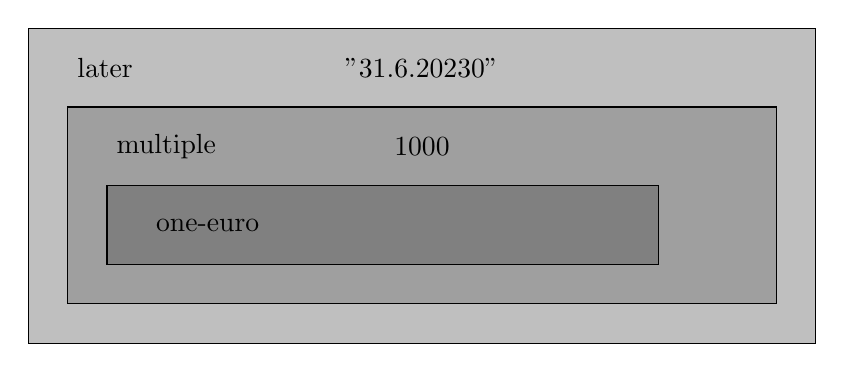
\begin{tikzpicture}
  \draw [fill=gray!50] (0, 0) rectangle (10, 4);
  \draw [fill=gray!75] (0.5, 0.5) rectangle (9.5, 3);
  \draw [fill=gray] (1, 1) rectangle (8, 2);
  \node [right] at (0.5, 3.5) {\lstinline{later}};
  \node at (5, 3.5) {\lstinline{"31.6.20230"}};
  \node [right] at (1, 2.5) {\lstinline{multiple}};
  \node at (5, 2.5) {\lstinline{1000}};
  \node [right] at (1.5, 1.5) {\lstinline{one-euro}};
\end{tikzpicture}
  
  \caption{Zero-Bond als Schichten dargestellt}
  \label{fig:zero-bond}
\end{figure}

\noindent Abbildung~\ref{fig:zero-bond} zeigt den Aufbau des
Zero-Bonds \lstinline{zero1} als ineinandergeschachtelte Schichten:
In den \lstinline{later}-Vertrag ist ein \lstinline{multiple}-Vertrag
eingeschachtelt, und dort wiederum der \lstinline{one-euro}-Vertrag.
Aus dieser Sicht ist der \lstinline{multiple}-Vertrag der
"<innere"> Vertrag des \lstinline{later}-Vertrags.

\paragraph{Verträge kombinieren}

Jetzt wo die Zero-Bonds erledigt sind, können wir überlegen, ob es
noch weitere Möglichkeiten geben sollte, Verträge herzustellen.  Immer
wenn Du Repräsentationen mit Kombinatoren baust, solltest Du nach
Möglichkeiten suchen, aus zwei Dingen ein größeres Ding zu bauen.

Beispiele für dieses Prinzip haben wir in diesem Kapitel schon mehrere
gesehen:
%
\begin{itemize}
\item Ein Hauptfluss und ein Nebenfluss werden zu einem Fluss
  kombiniert.
\item Zwei Bilder werden übereinander, nebeneinander und aufeinander
  zu einem Bild kombiniert.
\end{itemize}
%
Auf die Verträge bezogen bedeutet dies, dass wir zwei Verträge
zu einem zusammensetzen, der die Rechte und Pflichten von beiden kombiniert.
So könnte dies gehen:
%
\begin{lstlisting}
; Eine Kombinationsvertrag besteht aus:
; - Vertrag Nr. 1
; - Vertrag Nr. 2
\end{lstlisting}
%
Das sind wieder zusammengesetzte Daten mit zwei Selbstbezügen:
%
\begin{lstlisting}
(define-record-functions both
  make-both
  both?
  (both-contract-1 contract)
  (both-contract-2 contract))
\end{lstlisting}
%
Hier sind zwei Beispiele für \lstinline{both}:
%
\begin{lstlisting}
; Heute 100|\EUR{}|, später nochmal 100|\EUR{}|
(define both1 (make-both euro100 later1))
; Heute 200|\EUR{}|, später nochmal 200|\EUR{}|
(define both2 (make-both both1 later2))
\end{lstlisting}
%
Wir müssen noch die Definition von \lstinline{contract} erweitern:
%
\begin{lstlisting}
(define contract
  (signature (mixed one-euro multiple later both)))
\end{lstlisting}
%

\paragraph{Der kleinste Vertrag}

Es gibt noch ein weiteres Prinzip beim Repräsentieren mit
Kombinatoren: Suche immer nach dem \emph{kleinsten} möglichen
Baustein.  Wir haben ja schon einen ziemlich kleinen Baustein
definiert: \lstinline{one-euro}.  Aber oft ist der kleine Baustein
eine Variation von "<nichts">, und so ist es auch hier: Der kleinste
Vertrag ist einer ohne Rechte oder Pflichten.  Ihn sollten wir
unbedingt auch definieren~-- zunächst nur der Vollständigkeit halber,
aber später werden wir ihn tatsächlich noch brauchen.

Solch ein "<Nichts-Vertrag"> hat, wie \lstinline{one-euro} auch, keine
Eigenschaften.  Wir repräsentieren ihn aber, genau wie bei
\lstinline{one-euro}, durch einen Record, damit wir ihn mit Hilfe
seiner Signatur in die Definition von \lstinline{contract} einbauen
können:
%
\begin{lstlisting}
; Ein Nichts-Vertrag hat keine Eigenschaften
(define-record-functions nothing
  make-nothing
  nothing?)
\end{lstlisting}
%
Entsprechend erweitern wir \lstinline{contract}:
%
\begin{lstlisting}
(define contract
  (signature
   (mixed one-euro multiple later both nothing)))
\end{lstlisting}
%
In Aufgabe~\ref{aufgabe:give} auf Seite~\pageref{aufgabe:give} geht es
um noch einen weiteren Kombinator.

\paragraph{Verträge bewerten}

Wir haben viel Energie für die Repräsentation von Verträgen verwendet,
aber noch gar nichts damit gemacht.  Es fehlen noch ein paar saftige
Funktionen!

Wenn wir einen Vertrag haben, wollen wir vielleicht wissen, wieviel
Geld wir eigentlich insgesamt bekommen.  Das nehmen wir uns als erste
%% HK 2020-01-27: "jetzt" würde heissen "jetzt", also zu "diesem"
%% Zeitpunkt, das ist sicher nicht gemeint
Aufgabe vor.  Wir fangen an mit folgender Kurzbeschreibung:
%
\begin{lstlisting}
; Für einen Vertrag berechnen, wieviel Geld wir bekommen
\end{lstlisting}
%
In der Kurzbeschreibung tauchen die Begriffe "<Vertrag"> und "<Geld">
auf, das übersetzen wir in folgende Signatur:
%
\begin{lstlisting}
(: contract-payment (contract -> rational))
\end{lstlisting}
%
Die Funktion fasst alle Zahlungen zu einem Euro-Betrag zusammen,
Zinsen ignorieren wir.  Die Funktionsweise illustrieren wir wie immer
mit Testfällen.  Bei festen Euro-Beträgen ist recht klar, was
herauskommen muss:
%
\begin{lstlisting}
(check-expect (contract-payment euro100) 100)
(check-expect (contract-payment euro200) 200)
\end{lstlisting}
%
Die Beispiele \lstinline{later1} und \lstinline{later2} sind
verzögerte Verträge über \EUR{100} beziehungsweise \EUR{200}.  Die
Verzögerung spielt bei \lstinline{contract-payment} keine Rolle:
%
\begin{lstlisting}
(check-expect (contract-payment later1) 100)
(check-expect (contract-payment later2) 200)
\end{lstlisting}
%
Bei den beiden \lstinline{both}-Beispielen werden jeweils zwei
Zahlungen von \EUR{100} respektive \EUR{200} kombiniert:
%
\begin{lstlisting}
(check-expect (contract-payment both1) 200)
(check-expect (contract-payment both2) 400)
\end{lstlisting}
%
Die Schablone sieht so aus:
%
\begin{lstlisting}
(define contract-payment
  (lambda (contract)
    |\ldots|))
\end{lstlisting}
%
Da es sich bei der Definition von \lstinline{contract} um gemischte
Daten handelt, sieht die erste Schablone für
\lstinline{contract-payment} so aus:
%
\begin{lstlisting}
(define contract-payment
  (lambda (contract)
    (cond
      ((nothing? contract) |\ldots|)
      ((one-euro? contract) |\ldots|)
      ((multiple? contract) |\ldots|)
      ((later? contract) |\ldots|)
      ((both? contract) |\ldots|))))
\end{lstlisting}
%
Bei den einzelnen Fällen von \lstinline{contract} handelt es sich
jeweils um zusammengesetzte Daten, wir können also die Schablone um
die Anwendungen der Selektoren ergänzen, soweit es welche gibt:
%
\begin{lstlisting}
(define contract-payment
  (lambda (contract)
    (cond
      ((nothing? contract) |\ldots|)
      ((one-euro? contract) |\ldots|)
      ((multiple? contract)
       |\ldots|
       (multiple-number contract)
       (multiple-of contract)
       |\ldots|)
      ((later? contract)
       |\ldots|
       (later-date contract)
       (later-contract contract)
       |\ldots|)
      ((both? contract)
       |\ldots|
       (both-contract-1 contract)
       (both-contract-2 contract)
       |\ldots|))))
\end{lstlisting}
%
Es geht noch weiter:\\
\lstinline{(multiple-of contract)},\\
\lstinline{(later-contract contract)},\\
\lstinline{(both-contract-1 contract)}  und \lstinline{(both-contract-2 contract)} \\
sind allesamt
Selbstbezüge, wir können also dort rekursive Aufrufe hinschreiben:
%
\begin{lstlisting}
(define contract-payment
  (lambda (contract)
    (cond
      ((nothing? contract) |\ldots|)
      ((one-euro? contract) |\ldots|)
      ((multiple? contract)
       |\ldots|
       (multiple-number contract)
       (contract-payment (multiple-of contract))
       |\ldots|)
      ((later? contract)
       |\ldots|
       (later-date contract)
       (contract-payment (later-contract contract))
       |\ldots|)
      ((both? contract)
       |\ldots|
       (contract-payment (both-contract-1 contract))
       (contract-payment (both-contract-2 contract))
       |\ldots|))))
\end{lstlisting}
%
Damit ist die Schablone fertig und wir können versuche, für jeden Fall
etwas sinnvolles hinzuschreiben.  Bei den ersten beiden ist es nicht
so schwierig: Bei einem \lstinline{nothing}-Vertrag wird nichts
ausgezahlt, bei einem \lstinline{one-euro}-Vertrag wird ein \EUR{1}
ausgezahlt:
%
\begin{lstlisting}
(define contract-payment
  (lambda (contract)
    (cond
      ((nothing? contract) 0)
      ((one-euro? contract) 1)
      |\ldots|)))
\end{lstlisting}
%
Wir nehmen uns als nächstes den \lstinline{multiple}-Fall vor: Da
stehen in der Schablone schon:
\begin{itemize}
\item\lstinline{(multiple-number contract)}, also die \emph{Anzahl}
\item\lstinline{(contract-payment (multiple-of contract))}, also
  \emph{was bei einem ausgezahlt} wird
\end{itemize}
% 
Diese beiden Grüßen müssen wir miteinander multiplizieren, um die
Gesamtsumme zu berechnen, die ausgezahlt wird:
%
\begin{lstlisting}
(define contract-payment
  (lambda (contract)
    (cond
      |\ldots|
      ((multiple? contract)
       (* (multiple-number contract)
          (contract-payment (multiple-of contract))))
      |\ldots|)))
\end{lstlisting}
%
Nun ist der \texttt{later}-Fall an der Reihe.  Für
\lstinline{contract-payment} ist \lstinline{(later-date contract)},
also der Zeitpunkt, zu dem der Vertrag aktiv wird, irrelevant: Es geht
ja nur um den Betrag des "<inneren"> Vertrags, und der steht schon in
der Schablone:
%
\begin{lstlisting}
(define contract-payment
  (lambda (contract)
    (cond
      |\ldots|
      ((later? contract)
       (contract-payment (later-contract contract)))
      |\ldots|)))
\end{lstlisting}
%
Zu guter letzt kommt \lstinline{both}.  Die Zahlungen, die sich aus
den beiden Teilverträgen ergeben, stehen schon in der Schablone.  Wir
müssen sie lediglich addieren.  Die vollständige Funktion sieht dann
so aus:
%
\begin{lstlisting}
(define contract-payment
  (lambda (contract)
    (cond
      ((nothing? contract) 0)
      ((one-euro? contract) 1)
      ((multiple? contract)
       (* (multiple-number contract)
          (contract-payment (multiple-of contract))))
      ((later? contract)
       (contract-payment (later-contract contract)))
      ((both? contract)
       (+ (contract-payment (both-contract-1 contract))
          (contract-payment (both-contract-2 contract)))))))
\end{lstlisting}

\paragraph{Verträge verwalten}

Eine weitere nützliche Funktion von Verträgen betrifft die Entwicklung
eines Vertrags über die Zeit: Je länger ein Vertrag geschlossen ist,
desto mehr Zahlungen werden dadurch getätigt und entsprechend bleiben
weniger Zahlungen übrig.  Um das abzubilden, brauchen wir eine
Funktion, die ausrechnet, was von einem Vertrag nach einem bestimmten
Zeitpunkt noch übrigbleibt.  So könnte die Kurzbeschreibung lauten:
%
\begin{lstlisting}
; Was bleibt übrig, nachdem zu einem gegebenen Datum ausgezahlt wurde?
\end{lstlisting}
%
Um diese Funktion zu schreiben, müssen wir uns erst einmal überlegen,
wie dieser "<Rest"> von einem Vertrag repräsentiert werden kann.  Die
richtige Idee ist so einfach, dass es gar nicht so einfach ist, sie zu
sehen: Den "<Rest eines Vertrags"> können wir wieder als Vertrag
repräsentieren.  Wir müssen also keine neue Datenanalyse durchführen
und können mit der Signatur fortfahren.  Die Funktion braucht als
Eingabe einen Vertrag; als Ausgabe kommt der neue Vertrag heraus.
Außerdem brauchen wir noch das Datum, das in der Kurzbeschreibung
erwähnt wird:
%
\begin{lstlisting}
(: contract-rest (contract date -> contract))
\end{lstlisting}
%
Kommen wir zu einigen Testfällen: Die Verträge \lstinline{euro100} und
\lstinline{euro200} werden sofort ausgezahlt, da bleibt also nichts
mehr übrig:
%
\begin{lstlisting}
(check-expect (contract-rest euro100 date1) (make-nothing))
(check-expect (contract-rest euro200 date1) (make-nothing))
\end{lstlisting}
%
Das Beispiel \lstinline{later1} kommt zum Datum \lstinline{date1} zur
Auszahlung (der 26.~Juli 2019), ab diesem Datum ist also nichts mehr
übrig:
%
\begin{lstlisting}
(check-expect (contract-rest later1 date1) (make-nothing))
\end{lstlisting}
%
Der Beispielvertrag \lstinline{later2} hingegen wird erst zu
\lstinline{date2} ausgezahlt, das ist Weihnachten 2019.\footnote{Als
  dieses Kapitel geschrieben wurde, lag das noch in der Zukunft.}  Zum Zeitpunkt
\lstinline{date1} passiert deswegen noch nichts, der Vertrag
kommt also unverändert zurück:
%
\begin{lstlisting}
(check-expect (contract-rest later2 date1) later2)
\end{lstlisting}
%
Interesant wird es bei den \lstinline{both}-Verträgen.  Bei
\lstinline{both1} passiert der eine Teil sofort, der andere wird
bis \lstinline{date1} verzögert.  Zum Zeitpunkt \lstinline{date1}
bleibt allerdings von beiden Hälften nichts übrig:
%
\begin{lstlisting}
(check-expect (contract-rest both1 date1) (make-nothing))
\end{lstlisting}
%
Bei \lstinline{both2} bleibt allerdings zum Zeitpunkt
\lstinline{date1} noch etwas übrig, nämlich die "<rechte"> Hälfte,
\lstinline{later2}:
%
\begin{lstlisting}
(check-expect (contract-rest both2 date1) later2)
\end{lstlisting}
%
Aber zum Zeitpunkt \lstinline{date2} ist auch das perdu:
%
\begin{lstlisting}
(check-expect (contract-rest both2 date2) (make-nothing))
\end{lstlisting}
%
Wir schreiten nun zur Funktion selbst.  Hier das Gerüst:
%
\begin{lstlisting}
(define contract-rest
  (lambda (contract date)
    |\ldots|))
\end{lstlisting}
%
Die Eingabe-Signatur enthält ein \lstinline{contract}, wir können also
wieder die Schablone für gemischte Daten verwenden:
%
\begin{lstlisting}
(define contract-rest
  (lambda (contract date)
    (cond
      ((nothing? contract) |\ldots|)
      ((one-euro? contract) |\ldots|)
      ((multiple? contract) |\ldots|)
      ((later? contract) |\ldots|)
      ((both? contract) |\ldots|))))
\end{lstlisting}
%
Wir ergänzen als nächstes die Schablonen für die einzelnen Fälle, bei
denen es sich ja jeweils um zusammengesetzte Daten handelt:
%
\begin{lstlisting}
(define contract-rest
  (lambda (contract date)
    (cond
      ((nothing? contract) |\ldots|)
      ((one-euro? contract) |\ldots|)
      ((multiple? contract)
       |\ldots|
       (multiple-number contract)
       (multiple-of contract)
       |\ldots|)
      ((later? contract)
       |\ldots|
       (later-date contract)
       (later-contract contract)
       |\ldots|)
      ((both? contract)
       |\ldots|
       (both-contract-1 contract)
       (both-contract-2 contract)
       |\ldots|))))
\end{lstlisting}
%
%
Fast hätten wir es vergessen~-- in den Fällen für
\lstinline{multiple}, \lstinline{later} und \lstinline{both} gibt es
ja Selbstreferenzen und damit rekursive Aufrufe:
%
\begin{lstlisting}
(define contract-rest
  (lambda (contract date)
    (cond
      ((nothing? contract) |\ldots|)
      ((one-euro? contract) |\ldots|)
      ((multiple? contract)
       |\ldots|
       (multiple-number contract)
       (contract-rest (multiple-of contract) date)
       |\ldots|)
      ((later? contract)
       |\ldots|
       (later-date contract)
       (contract-rest (later-contract contract) date)
       |\ldots|)
      ((both? contract)
       |\ldots|
       (contract-rest (both-contract-1 contract) date)
       (contract-rest (both-contract-2 contract) date)
       |\ldots|))
    |\ldots|
    (date-year date)
    (date-month date)
    (date-day date)
    |\ldots|))
\end{lstlisting}
%
Wir können außerdem noch die Schablone für \lstinline{date} bemühen,
wobei es sich zum zusammengesetzte Daten handelt.  Das Datum ist nur
im \lstinline{later}-Fall relevant~-- wir füllen die Schablone aus,
wenn wir zu diesem Fall kommen.

Wir fangen wieder mit den einfachen Fällen an.  Bei
\lstinline{nothing} und \lstinline{one-euro} bleibt jeweils nichts
übrig:
%
\begin{lstlisting}
(define contract-rest
  (lambda (contract date)
    (cond
      ((nothing? contract) (make-nothing))
      ((one-euro? contract) (make-nothing))
      |\ldots|)))
\end{lstlisting}
%
\begin{aufgabeinline}
  Sind beide Fälle schon durch Testfälle abgedeckt?  Wenn nicht,
  schreibe einen!
\end{aufgabeinline}
%
Als nächstes ist \lstinline{multiple} an der Reihe.  Der rekursive
Aufruf aus der Schablone beantwortet die folgende Frage: "<Wieviel ist
von \emph{einem} Vertrag nach dem Datum noch übrig?"> Wenn wir mit $n$
das Ergebnis von \lstinline{(multiple-number contract)} bezeichnen,
dann müssen wir die Frage beantwortenm, wieviel von $n$
Verträgen übrig bleibt.  Im übertragenen Sinne futtern $n$ Esser in
der Mensa an jeweils der gleichen Portion Brei, werden aber
unterbrochen. Wenn wir wissen, wieviel von einer Portion jeweils übrigbleibt,
wieviel bleibt dann insgesamt übrig?  Wir müssen wieder mit $n$
multiplizieren:
%
\begin{lstlisting}
(define contract-rest
  (lambda (contract date)
    (cond
      |\ldots|
      ((multiple? contract)
       (make-multiple (multiple-number contract)
                      (contract-rest (multiple-of contract) date)))
      |\ldots|)))
\end{lstlisting}
%
Als nächstes ist der \lstinline{later}-Fall dran.  Der rekursive
Aufruf beantwortet die Frage, was von dem Vertrag übrigbleibt, falls
das Datum \lstinline{date} schon vorbei beziehungsweise gerade heute
ist.  Wenn \lstinline{date} noch in der Zukunft liegt, passiert gar
nichts und die Funktion sollte den gesamten Vertrag
\lstinline{contract} zurückliefern.

Das heißt, das \lstinline{date} in zwei Klassen zerfällt, nämlich (a)
vor oder gleich dem Datum \lstinline{(later-date contract)} oder (b)
danach.  Wir brauchen also eine Verzweigung danach, und dazu müssen
wir die beiden Daten miteinander vergleichen.  Diese Aufgabe ist
hinreichend kompliziert, dass wir sie zurückstellen und uns
fest vornehmen, später eine Funktion mit folgender Kurzbeschreibung
und Signatur zu schreiben:
%
\begin{lstlisting}
; Ist ein Datum früher als ein anderes?
(: date<=? (date date -> boolean))
\end{lstlisting}
%
Mit Hilfe dieser Funktion können wir den \lstinline{later}-Fall
folgendermaßen fertigstellen:
%
\begin{lstlisting}
(define contract-rest
  (lambda (contract date)
    (cond
      |\ldots|
      ((later? contract)
       (if (date<=? (later-date contract) date)
           (contract-rest (later-contract contract) date)
           contract))
      |\ldots|)))
\end{lstlisting}
%
Wir haben dabei etwas geschummelt und uns darum gedrückt, die
Schablone für \lstinline{date} auszufüllen.  Das müssen wir bei
\lstinline{date<=?} nachholen.

Es bleibt der Fall für \lstinline{both}.  Die rekursiven Aufrufe aus der
Schablone liefern, was vom "<linken"> beziehungsweise "<rechten">
Vertrag übriggeblieben ist.  Wir müssen die Ergebnisse nur wieder
zusammensetzen:
%
\begin{lstlisting}
(define contract-rest
  (lambda (contract date)
    (cond
      |\ldots|
      ((both? contract)
       (make-both (contract-rest (both-contract-1 contract) date)
                  (contract-rest (both-contract-2 contract) date))))))
\end{lstlisting}
%
Fertig!

Also fast: Wir müssen ja noch die Funktion \lstinline{date<=?}
schreiben.  Für einen Teil davon spannen wir Dich ein:
%
\begin{aufgabeinline}
  Schreibe ausreichende Testfälle für \lstinline{date<=?}!
\end{aufgabeinline}
%
Hier ist das Gerüst:
%
\begin{lstlisting}
(define date<=?
  (lambda (date1 date2)
    |\ldots|))
\end{lstlisting}    
%
Das es sich sowohl bei \lstinline{date1} als auch \lstinline{date2} um
zusammengesetzte Daten handelt
%
\begin{lstlisting}
(define date<=?
  (lambda (date1 date2)
    |\ldots|
    (date-year date1) (date-year date2)
    (date-month date1) (date-month date2)
    (date-day date1) (date-day date2)
    |\ldots|))
\end{lstlisting}    
%
Um den Rumpf richtig hinzubekommen, müssen wir sorgfältig alle
möglichen Fälle abarbeiten.  Zunächst müssen wir die beiden
Jahreszahlen vergleichen~-- wenn sie bei \lstinline{date1} und
\lstinline{date2} unterschiedlich sind, so steht das Ergebnis fest.
Wenn nicht, so muss die Funktion die Monate vergleichen und
schließlich die Tage.  Das sieht am Ende so aus:
%
\begin{lstlisting}
(define date<=?
  (lambda (date1 date2)
    (cond
      ((< (date-year date1) (date-year date2)) #t)
      ((> (date-year date1) (date-year date2)) #f)
      ((< (date-month date1) (date-month date2)) #t)
      ((> (date-month date1) (date-month date2)) #f)
      ((< (date-day date1) (date-day date2)) #t)
      ((> (date-day date1) (date-day date2)) #f)
      (else #t))))
\end{lstlisting}
    
\paragraph{Verträge vereinfachen}

Leider ist der Code für die \lstinline{contract-rest}-Funktion zwar
vollständig, funktioniert aber nicht wie erwartet: Die Tests schlagen
fehl, und zwar fast alle!  Wie kann das sein?  Hier ist
der erste:
%
\begin{lstlisting}
(check-expect (contract-rest euro100 date1) (make-nothing))
\end{lstlisting}
%
Hier ist die Meldung vom Fehlschlag:
%
\begin{alltt}
Der tatsächliche Wert \textcolor{blue}{#<record:multiple 100 #<record:nothing>>}
ist nicht der erwartete Wert \textcolor{blue}{#<record:nothing>}.
\end{alltt}
%
Was ist passiert?  Zur Erinnerung, der Vertrag \lstinline{euro100} ist
so definiert:
%
\begin{lstlisting}
(define euro100 (make-multiple 100 (make-one-euro))) 
\end{lstlisting}
%
Die \lstinline{contract-rest}-Funktion hat erst einmal berechnet, was
von dem einen Euro übriggeblieben ist und vom Rest dann 100 Stück
zurückgegeben: 100 Stück von nichts.  Das Ergebnis ist ja auch
formal korrekt, aber eben nicht wie vom Testfall erwartet.
Unpraktisch ist es auf jeden Fall:
%
\begin{aufgabeinline}
  Finde noch drei weitere komplizierte Wege, "<Verträge über nichts">
  aufzuschreiben.
\end{aufgabeinline}
%
Um das Problem zu vermeiden, wäre es gut, wenn das Programm Verträge
über "<$n$ mal nichts"> gar nicht erst konstruieren würden.  Dafür
müssen wir beim Konstruktor \lstinline{make-multiple} ansetzen.  Wenn
der auf einen \lstinline{nothing}-Vertrag angewendet wird, muss das
Ergebnis auch wieder ein \lstinline{nothing}-Vertrag sein.  Um das zu
erreichen, müssen wir \lstinline{make-multiple} umdefinieren.  Da die
Definition von \lstinline{make-multiple} von
\lstinline{define-record-functions} erledigt wird, wenden wir einen
Trick an und benennen den Konstruktor erst einmal um, in dem wir die
Record-Definition ändern:
%
\begin{lstlisting}
(define-record-functions multiple
  really-make-multiple
  multiple?
  (multiple-number   rational)
  (multiple-of       contract))
\end{lstlisting}
%
Der Name \lstinline{really-make-multiple} ist reine Konvention~--
solange der Name nur anders ist als \lstinline{make-multiple}!  Als
nächstes definieren wir eine neue Funktion mit dem alten Namen und dem
gleichen Vertrag.  Hier Kurzbeschreibung, Signatur und ein Testfall,
der gerade \lstinline{euro100} entspricht:
%
\begin{lstlisting}
; multiple-Vertrag konstruieren, dabei vereinfachen
(: make-multiple (rational contract -> contract))

(check-expect (make-multiple 100 (make-nothing)) (make-nothing))
\end{lstlisting}
%
Hier ist das Gerüst für die Funktion:
%
\begin{lstlisting}
(define make-multiple
  (lambda (factor contract)
    |\ldots|))
\end{lstlisting}
%
Die Eingabe \lstinline{contract} zerfällt nun in zwei Fälle:
\lstinline{nothing}-Verträge und alle anderen.  Im ersten Fall geben
wir wieder einen \lstinline{nothing}-Vertrag zurück, im zweiten Fall
rufen wir den richtigen Konstruktor auf:
%
\begin{lstlisting}
(define make-multiple
  (lambda (factor contract)
    (if (nothing? contract)
        (make-nothing)
        (really-make-multiple factor contract))))
\end{lstlisting}
%
Damit funktionieren schonmal die ersten beiden Testfälle, die
ursprünglich fehlgeschlagen sind.  Es bleiben aber noch weitere.  Der erste
ist dieser hier:
%
\begin{alltt}
Der tatsächliche Wert #<record:both \textcolor{blue}{#<record:nothing> #<record:nothing>>}
ist nicht der erwartete Wert \textcolor{blue}{#<record:nothing>}.
\end{alltt}
%
Das deutet auf ein analoges Problem wie bei \lstinline{multiple} hin:
Nichts und nochmal nichts ist eben nichts, aber der Konstruktor von
\lstinline{both} weiß das nicht.  Wir wenden den gleichen Trick an und
benennen zunächst den Konstruktor um:
%
\begin{lstlisting}
(define-record-functions both
  really-make-both
  both?
  (both-contract-1 contract)
  (both-contract-2 contract))  
\end{lstlisting}
%
Als nächstes definieren wir einen neuen Konstruktor selber:
%
\begin{lstlisting}
; Kombinationsvertrag konstruieren, dabei vereinfachen
(: make-both (contract contract -> contract))

(check-expect (make-both (make-nothing) (make-nothing)) (make-nothing))
\end{lstlisting}
%
Durch diesen Testfall ist "<nichts und nichts"> abgedeckt.  Das können
wir aber noch etwas verallgemeinern.  Das illustrieren am besten die
folgenden Testfälle, bei denen jeweils nur die linke beziehungsweise
rechte Seite des \lstinline{both}-Vertrags nichts ist:
%
\begin{lstlisting}
(check-expect (make-both (make-one-euro) (make-nothing)) (make-one-euro))
(check-expect (make-both (make-nothing) (make-one-euro)) (make-one-euro))
\end{lstlisting}
%
Hier ist das Gerüst zur Funktion:
%
\begin{lstlisting}
(define make-both
  (lambda (contract-1 contract-2)
    |\ldots|))
\end{lstlisting}
%
Die Eingaben zerfallen in drei Klassen, nämlich wenn
\lstinline{contract-1} nichts ist, wenn \lstinline{contract-2} nichts
ist und alle anderen.  Entsprechend brauchen wir eine Verzweigung mit
drei Zweigen:
%
\begin{lstlisting}
(define make-both
  (lambda (contract-1 contract-2)
    (cond
      ((nothing? contract-1) contract-2)
      ((nothing? contract-2) contract-1)
      (else
       (really-make-both contract-1 contract-2)))))
\end{lstlisting}
%
Und nun endlich verlaufen alle Tests erfolgreich.

Die Funktionen \lstinline{make-multiple} und \lstinline{make-both},
welche die ursprünglichen Konstruktoren gleichen Namens ersetzen und
bei der Konstruktion die entstehenden Verträge gleich schon etwas
vereinfachen heißen auch \textit{smart constructors}.\index{smart constructor}

\paragraph{Kombinatorrepräsentationen finden} Die Autoren des Papers über Finanzverträge
haben Monate gebraucht, um die beschriebene elegante Repräsentation zu
finden.  Sie sind nach zwei Prinzipien vorgegangen:
%
\begin{itemize}
\item Sie haben Finanzverträge in ihre kleinsten Bestandteile zerlegt.
\item Sie haben nach Kombinatoren für Finanzverträge gesucht und
  welche gefunden, entsprechend Mantra~\ref{mantra:kombinator} auf Seite~\pageref{mantra:kombinator}.
\end{itemize}
%
Die Prinzipien sind auf viele andere Problemstellungen übertragbar.

\section*{Aufgaben}

\begin{aufgabe}
  Schreibe einen sinnvollen \textit{smart constructor} für
  \lstinline{later}-Verträge.
\end{aufgabe}

\begin{aufgabe}
  Betrachte folgenden Vertrag:
  %
\begin{lstlisting}
(make-multiple 100 (make-multiple 100 (make-one-euro)))    
\end{lstlisting}
%
Kann dieser Vertrag vereinfacht werden?  Wenn ja, erweitere den
entsprechenden \textit{smart constructor}.
\end{aufgabe}

\begin{aufgabe}\label{aufgabe:give}
  Füge eine weitere Klasse von Verträgen hinzu, die
  \lstinline{give}-Verträge: Ein \lstinline{give}-Vertrag dreht alle
  Zahlungen um, die sich aus einem Vertrag ergeben.  Das heißt, ein
  \lstinline{give}-Vertrag von \EUR{1} führt dazu, dass der
  Vertragsinhaber dem Vertragspartner \EUR{1} \emph{geben} muss und
  nicht bekommt.  Erweitere die beiden Funktionen, so dass sie auch
  mit \lstinline{give}-Verträgen klarkommen.  Benutze, um Zahlungen
  "<in die andere Richtung"> zu repräsentieren, ein negatives
  Vorzeichen.
\end{aufgabe}

\begin{aufgabe}
  Die Funktionen \lstinline{contract-payment} und
  \lstinline{contract-rest} passen nicht so recht zusammen: Die eine
  berechnet \emph{alle} Zahlungen, die anderen den Rest eines Vertrags
  ab einem bestimmten Zeitpunkt.  Schreibe eine Funktion
  \lstinline{contract-payment-until}, die alle Zahlungen bis zu einem
  bestimmten Zeitpunkt berechnet!
\end{aufgabe}

\begin{aufgabe}\label{aufgabe:aufzaehlung-vs-nullstellig}
  Statt nullstelliger zusammengesetzter Daten wie \lstinline{nothing}
  oder \lstinline{one-euro} könnte man theoretisch auch~-- wie bei
  Aufzählungen~-- feste Zeichenketten wie \lstinline{"nothing"} und
  \lstinline{"one-euro"} verwenden.  Versuch dies umzusetzen!
\end{aufgabe}

%%% Local Variables: 
%%% mode: latex
%%% TeX-master: "i1"
%%% End: 


